\documentclass[10pt,a4paper]{article}
\usepackage[UTF8,fontset = windows]{ctex}
\setCJKmainfont[BoldFont=黑体,ItalicFont=楷体]{华文中宋}
\usepackage{amssymb,amsmath,amsfonts,amsthm,mathrsfs,dsfont,graphicx}
\usepackage{ifthen,indentfirst,enumerate,color,titletoc}
\usepackage{tikz}
\usepackage{makecell}
\usepackage{longtable}
\usetikzlibrary{arrows,calc,intersections,patterns}
\usepackage[bf,small,indentafter,pagestyles]{titlesec}
\usepackage[top=1in, bottom=1in,left=0.8in,right=0.8in]{geometry}
\renewcommand{\baselinestretch}{1.65}
\newtheorem{defi}{定义~}
\newtheorem{eg}{例~}
\newtheorem{ex}{~}
\newtheorem{rem}{注~}
\newtheorem{thm}{定理~}
\newtheorem{coro}{推论~}
\newtheorem{axiom}{公理~}
\newtheorem{prop}{性质~}
\newcommand{\blank}[1]{\underline{\hbox to #1pt{}}}
\newcommand{\bracket}[1]{(\hbox to #1pt{})}
\newcommand{\onech}[4]{\par\begin{tabular}{p{.9\textwidth}}
A.~#1\\
B.~#2\\
C.~#3\\
D.~#4
\end{tabular}}
\newcommand{\twoch}[4]{\par\begin{tabular}{p{.46\textwidth}p{.46\textwidth}}
A.~#1& B.~#2\\
C.~#3& D.~#4
\end{tabular}}
\newcommand{\vartwoch}[4]{\par\begin{tabular}{p{.46\textwidth}p{.46\textwidth}}
(1)~#1& (2)~#2\\
(3)~#3& (4)~#4
\end{tabular}}
\newcommand{\fourch}[4]{\par\begin{tabular}{p{.23\textwidth}p{.23\textwidth}p{.23\textwidth}p{.23\textwidth}}
A.~#1 &B.~#2& C.~#3& D.~#4
\end{tabular}}
\newcommand{\varfourch}[4]{\par\begin{tabular}{p{.23\textwidth}p{.23\textwidth}p{.23\textwidth}p{.23\textwidth}}
(1)~#1 &(2)~#2& (3)~#3& (4)~#4
\end{tabular}}
\begin{document}
\begin{enumerate}[1.]
\item 请根据图中的函数图像, 将下列数值按从小到大的顺序排列:\blank{50}.
\begin{center}
    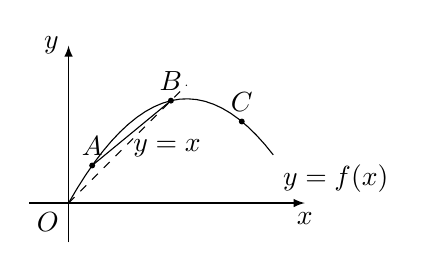
\begin{tikzpicture}[>=latex]
        \draw [->] (-0.5,0) -- (3,0) node [below] {$x$};
        \draw [->] (0,-0.5) -- (0,2) node [left] {$y$};
        \draw (0,0) node [below left] {$O$};
        \draw [domain = 0:2.6, name path = curve] plot (\x,{\x*(3-\x)/1.7}) node [below right] {$y=f(x)$};
        \draw [dashed] (0,0) -- (1.5,1.5);
        \filldraw (1.3,1.3) circle (0.03) node [above] {$B$} -- (0.3,{0.3*2.7/1.7}) circle (0.03) node [above] {$A$};
        \filldraw (2.2,{2.2*0.8/1.7}) circle (0.03) node [above] {$C$};
        \draw (0.7,0.7) node [right] {$y=x$};
    \end{tikzpicture}    
\end{center}
\textcircled{1} 曲线在点$A$处切线的斜率;\\
\textcircled{2} 曲线在点$B$处切线的斜率;\\
\textcircled{3} 曲线在点$C$处切线的斜率;\\
\textcircled{4} 割线$AB$的斜率;\\
\textcircled{5} 数值$0$;\\
\textcircled{6} 数值$1$.
\item 2.已知$f(x)=\sqrt{x}$, $g(x)=kx^x$.\\
(1) 求曲线$y=f(x)$在点$(4,2)$处的切线方程;\\
(2) 若曲线$y=g(x)$经过点$(4,2)$, 求它与(1)中切线的另一个交点.
\item 从桥上将一小球掷向空中, 小球相对于地面的高度$h$(单位: $\text{m}$)和时间$t$(单位: $\text{s}$)近似满足函数关系$h=-5t^2+15t+12$. 问:\\
(1) 小球的初始高度是多少?\\
(2) 小球在$t=0$到$t=1$这段时间内的平均速度是多少?\\
(3) 小球在$t=1$时的瞬时速度是多少?\\
(4) 小球所能达到的最大高度是多少? 何时达到?
\item 已知$f(x)=lnx$, $g(x)=\mathrm{e}^x$, 计算下列函数$y=h(x)$在点$x=1$处的导数值:\\
(1) $h(x)=3f(x)-5g(x)$;\\
(2) $h(x)=f(x)g(x)$;\\
(3) $h(x)=\dfrac{f(x)}{g(x)}$;\\
(4) $h(x)=f(2x+1)+g(3x-1)$.
\item 计算下列函数$y=f(x)$的导数, 其中:\\
(1) $f(x)=\dfrac\pi 2+\sin(-x)$;\\
(2) $f(x)=\sqrt[3]{x}-\dfrac{1}{x^3}$;\\
(3) $f(x)=(\dfrac 12 x-5)(3-4x)$;\\
(4) $f(x)=\dfrac{\cos x}{x^2}$.
\item 求下列函数$y=f(x)$的单调区间和极值点, 其中:
(1) $f(x)=\dfrac 23 x-1$;\\
(2) $f(x)=2+x-x^2$;\\
(3) $f(x)=x^3+x^2-8x+7$.
\item 借助求导数的结果, 求下列函数$y=f(x)$在给定区间上的最大值和最小值, 其中:\\
(1) $f(x)=\dfrac 23 x-1, \  x\in [0, 3]$;\\
(2) $f(x)=2+x-x^2, \ x\in [-1, 1]$;\\
(3) $f(x)=x^3+x^2-8x+7, \ x\in [-3, 3]$.
\item 已知$y=f'(x)$的图像如图所示, 求函数$y=f(x)$在$(-2,2)$上的单调区间和极值点.
\begin{center}
    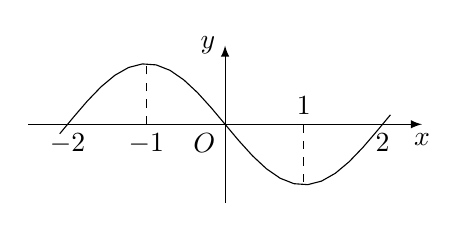
\begin{tikzpicture}[>=latex]
        \draw [->] (-2.5,0) -- (2.5,0) node [below] {$x$};
        \draw [->] (0,-1) -- (0,1) node [left] {$y$};
        \draw (0,0) node [below left] {$O$};
        \draw [domain = -2.1:2.1] plot (\x, {-sin(\x*90)/1.3});
        \draw [dashed] (-1,0) node [below] {$-1$} -- (-1,{1/1.3}) (1,0) node [above] {$1$}-- (1,{-1/1.3});
        \draw (-2,0) node [below] {$-2$} (2,0) node [below] {$2$};
    \end{tikzpicture}
\end{center}
\item 若直线$y=x$是曲线$y=x^3-3x^2+ax$的切线, 求$a$的值.
\item 设函数$y=x^3+ax^2+bx+c$的图像与$y=0$在原点相切, 若函数的极小值为$-4$, 求函数的表达式与单调减区间.
\item 某种型号的汽车在匀速行驶中每小时的耗油量$y$(单位: $\text{L}$)关于行驶速度$x$(单位: $\text{km}/\text{h}$)满足函数关系$y=\dfrac 1{128000}x^3-\dfrac 3{80}x+8 \ (0<x\le 120)$. 已知甲、乙两地相距$100\text{km}$. 问: 当汽车保持怎样的速度匀速行驶时, 从甲地到乙地的耗油量最小?
\item 要建造一个给定容积$V$的圆柱体蓄水池, 已知池底单位造价为池侧面单位造价的$2$倍. 问: 应如何选择蓄水池的底面半径$r$和高$h$, 才能使总造价最低?
\item 已知某厂生产一种产品的总成本$C$(单位: 万元)与产品件数$x$满足函数关系$C=1200+\dfrac2 {75}x^3$, 产品单价$P$(单位: 万元)和产品件数$x$满足函数关系$P^2=\dfrac{250000}x$. 问: 产量为多少件时, 总利润最大?
\item 讨论函数$y=x^3+ax+b$的单调性(可借助信息技术工具).
\item 判断方程$x^3+ax+b=0$有几个实根(可借助信息技术工具).

\item 如图, 用$6$种不同的颜色将$A$、$B$、$C$三个区域涂色, 每个区域涂上一种颜色, 且有公共边的区域不能涂同一种颜色. 问: 不同的涂色方法共有多少种?
\begin{center}
    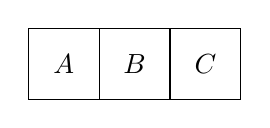
\begin{tikzpicture}[scale = 0.6]
        \draw (0,0) rectangle (4.5,1.5);
        \draw (1.5,0) -- (1.5,1.5) (3,0) -- (3,1.5);
        \draw (0.75,0.75) node {$A$} (2.25,0.75) node {$B$} (3.75,0.75) node {$C$};
    \end{tikzpicture}
\end{center}
\item $5$个工程队分别承建某项工程的$5$个不同的子项目, 每个工程队各承建其中的$1$项, 且甲工程队不能承建$1$号子项目. 问: 不同的承建方案有多少种?
\item 从$0$、$1$、$2$、$3$、$4$、$5$六个数字中任取四个数字, 可以组成多少个没有重复数字、且为奇数的四位数?
\item 解关于正整数$x$的方程: $11\mathrm{C}_x^3=24\mathrm{C}_{x+1}^2$.
\item 已知$(x^2+\dfrac 1x)^n$的二项展开式的各项系数之和为$32$, 求该二项展开式中$x$的系数.
\item 若$(1-2x)^4=a_0+a_1x+a_2x^2+a_3x^3+a_4x^4$, 求$|a_0|+|a_1|+|a_3|$的值.
\item 若$(x^6+\dfrac 1{x\sqrt x})^n$的二项展开式中含有常数项, 求$n$的最小值.
\item $7$名学生站成一排拍毕业纪念照, 其中甲必须站在正中间, 并且乙、丙$2$名学生要站在一起. 问: 有多少种不同的排法?
\item 将$5$个不同的小球分别放到$3$个不同的盒子中, 要求每个盒子都不空. 问: 有多少种不同的放法?
\item 从$7$名男乒乓球队员、$5$名女乒乓球队员中任选$4$名进行男女混合双打, 不同的分组方法有多少种?
\item $3$名男生、$4$名女生排成一行. 在下列要求下, 分别求不同排列方法的种数:\\
(1) 甲不在最左边, 乙不在最右边;\\
(2) 男生必须排在一起;\\
(3) 男生和女生相间排列;\\
(4) 在甲、乙两人中间必须有$3$人.
\item 一个口袋内有$4$个不同的红球、$6$个不同的白球.\\
(1) 从中任取$4$个球, 红球的个数不比白球少的取法有多少种?\\
(2) 若取一个红球记$2$分, 取一个白球记$1$分. 从中任取$5$个球, 使总分不少于$7$分的取法有多少种?
\item 设$(2-\sqrt 3x)^{100}=a_0+a_1x+a_2x^2+\cdots+a_{100}x^{100}$, 求下列各式的值:\\
(1) $a_0$;\\
(2) $a_1+a_3+a_5+\cdots+a_{99}$;\\
(3) $(a_0+a_2+a_4+\cdots+a_{100})^2-(a_1+a_3+\cdots+a_{99})^2$. \item 利用二项式定理, 求$55^{55}$被$8$除所得的余数.
\item 设集合$A$是由所有满足下面条件的有序数组$(x_1,x_2,x_3,x_4,x_5)$构成的: 每一个元素$x_i$等于$0$、$1$、$-1$中之一, 其中$i=1,2,3,4,5$. 那么集合$A$中满足条件``$1\le |x_1|+|x_2|+|x_3|+|x_4|+|x_5|\le 3$''的元素有多少个?
\item 利用二项式定理证明: 对于任意正整数$n$, $\dfrac1{\sqrt 5}[(2+\sqrt 5)^n-(2-\sqrt 5)^n]$都是正整数. 

\item 掷黄、白两颗骰子, 当黄色骰子的点数为$4$或$6$时, 求两颗骰子的点数之积大于$20$的概率.
\item 连续掷一颗骰子两次, 已知第一次掷出的是偶数点. 求第二次也掷出偶数点的
概率. 
\item 在$5$道题中有$3$道数学题和$2$道语文题. 如果不放回地依次抽取$2$道题, 求:\\
(1) 第$1$次抽到数学题的概率;\\
(2) 第$1$次和第$2$次都抽到数学题的概率;\\
(3) 在第$1$次抽到数学题的条件下, 第$2$次也抽到数学题的概率.
\item 已知随机变量$X$的分布为$\begin{pmatrix} -1 & 0 & 1 \\ a & b & c\end{pmatrix}$. 若$E[X]=\dfrac 13$, $D[X]=\dfrac 59$, 求$a$、$b$、$c$的值.
\item 同时抛掷两枚相同的均匀硬币, 设随机变量$X=1$表示结果中有正面朝上, $X=0$表示结果中没有正面朝上. 求$E[X]$及$D[X]$.
\item 从$4$名男生和$2$名女生中任选$3$人参加演讲比赛, 设随机变量$X$表示所选$3$人中女生的人数. 求:\\
(1) $X$的分布;\\
(2) $X$的期望与方差;\
(3) ``所选$3$人中女生人数$X\le 1$''的概率.
\item 一批产品的二等品率为$0.02$. 从这批产品中每次随机取一件, 有放回地抽取$100$次. 用$X$表示抽到的二等品件数, 求$D[X]$.
\item 袋中有$10$个大小与质地相同的球, 其中$7$个是红球. 从中任取$5$个球, 求取出的球中红球个数$X$的分布.
\item 某人提出一个问题, 甲先答, 答对的概率为$0.4$. 若甲答错, 则由乙答, 乙答对的概率为$0.5$. 求该问题由乙答对的概率.
\item $100$件产品中有$5$件次品, 不放回地抽取两次, 每次抽$1$件. 已知第一次抽出的是次品, 求第二次抽出正品的概率.
\item 盒中有大小与质地相同的$25$个球, 其中$10$个白球、$5$个黄球、$10$个黑球. 从盒中任意取出$1$个球, 已知它不是黑球, 求它是黄球的概率.
\item 在$1$、$2$、$3$、$\cdots$、$9$这$9$个自然数中, 任取$3$个数.\\
(1) 求这$3$个数中恰有$1$个是偶数的概率;\\
(2) 设$X$为这$3$个数中两数相邻的组数(例如, 若取出的数为$1$、$2$、$3$, 则有两组相邻的数$1$、$2$和$2$、$3$, 此时$X$的值为$2$), 求随机变量$X$的分布及期望.
\item 口袋里装有大小与质地相同的$4$个红球和$8$个白球, 甲、乙两人依下面的规则从袋中有放回地摸球, 每次摸$1$个球. 规则如下: 若一方摸出$1$个红球, 则此人继续下一次摸球; 若一方摸出$1$个白球, 则由对方接替下一次摸球. 假设每次摸球相互独立, 且由甲进行第一次摸球. 求在前三次摸球中, 甲摸得红球的次数$X$的分布及期望.
\item 在一个游戏中, 每次输赢的概率都是$\dfrac 12$. 甲的策略是: 第一次押$1$元, 如果赢, 就结束; 如果输, 押$2$元再来一次, 无论输赢都结束. 乙的策略是: 押$1$元, 无论输赢都结束.\\
(1) 求甲赢的概率与乙赢的概率;\\
(2) 用$X$、$Y$分别表示甲、乙最终赢得的金额(即所押金额), 求它们的分布与期望;\\
(3) 比较甲与乙的策略.
\item 设有两个罐子, $A$罐中放有$2$个白球、$1$个黑球, $B$罐中放有$3$个白球, 这些球的大小与质地相同. 现在从两个罐子中各摸$1$个球进行交换, 求这样交换$3$次后, 黑球还在$A$罐中的概率. 交换$n$次后呢?
\item 有一种骰子游戏, 某人掷两颗骰子, 若掷出的点数之和是$7$或$11$, 则赢; 若掷出的点数之和是$2$、$3$或$12$, 则输; 若掷出其他的点数和, 则记下这个数, 继续掷这两颗骰子, 直到掷出的点数和是这个记下的数或者$7$为止, 若是这个记下的数, 则赢, 若是$7$, 则输. 求此人赢的概率是多少.
\item 在研究硝酸钠的可溶性程度时, 观测它在不同温度(单位: $^\circ\text{C}$)$100\text{g}$的水中的溶解度(单位: $\text{g}$), 得到如下观测结果:
\begin{center}
    \begin{tabular}{|c|c|c|c|c|c|c|c|c|}
        \hline
        温度$x/^\circ\text{C}$ & $10$ & $25$ & $40$ & $50$ & $55$ & $60$ & $65$ & $75$ \\ \hline
        溶解度$y/\text{g}$ & $81$ & $92$ & $104$ & $114$ & $117$ & $124$ & $130$ & $150$ \\ \hline
    \end{tabular}
\end{center}
由此得到回归直线的斜率是\blank{50}.
\item 若对具有线性相关关系的两个变量建立的回归方程为$y=-0.960x+3.134$, 则当$x=50$时, $y$的估计值为\blank{50}.
\item 某产品的广告费投入与销售额的统计数据如下表所示.
\begin{center}
    \begin{tabular}{|c|c|c|c|c|}
        \hline
        广告费$x/$万元 & $4$ & $2$ & $3$ & $5$ \\ \hline
        销售额$y/$万元 & $49$ & $26$ & $39$ & $54$ \\ \hline   
    \end{tabular}
\end{center}
根据上表建立的回归方程$y=\hat ax+\hat b$中, $\hat a=9.4$. $9.4$的实际意义是什么?
\item 经过分层抽样得到$16$名学生高一和高二结束时的数学考试成绩(满分: $100$分), 如下表所示.
\begin{center}
    \begin{tabular}{|c|c|c|c|c|c|c|c|c|}
        \hline
        学生编号& $1$ & $2$ & $3$ & $4$ & $5$ & $6$ & $7$ & $8$ \\ \hline 
        高一& $84$ & $85$ & $71$ & $74$ & $60$ & $58$ & $51$ & $82$ \\ \hline 
        高二& $84$ & $88$ & $72$ & $73$ & $68$ & $62$ & $60$ & $85$ \\ \hline \hline
        学生编号& $9$ & $10$ & $11$ & $12$ & $13$ & $14$ & $15$ & $16$ \\ \hline 
        高一& $87$ & $69$ & $79$ & $80$ & $83$ & $84$ & $63$ & $54$ \\ \hline 
        高二& $88$ & $73$ & $84$ & $82$ & $83$ & $83$ & $66$ & $67$ \\ \hline
    \end{tabular}
\end{center}
(1) 绘制这些成对数据的散点图;\\
(2) 计算学生高一和高二数学成绩的相关系数. 根据此相关系数, 你能得出什么
结论?
\item 通过随机询问$72$名大学生在购买食品时是否读营养说明, 得到如下列联表:
\begin{center}
    \begin{tabular}{|c|c|c|c|}
        \hline
        表头 & 男 & 女 & 总计\\ \hline 
        读营养说明& $28$& $16$& $44$\\ \hline 
        不读营养说明& $8$& $20$& $28$\\ \hline 
        总计& $36$& $36$& $72$\\ \hline 
    \end{tabular}
\end{center}
根据表中的数据回答: 是否有$95\%$的把握判定性别与读营养说明之间有关系?
\item 某人对一地区近几年的年人均可支配收入$x$(单位: 千元)与年人均消费支出$y$(单位: 千元)进行统计调查, 发现$y$与$x$具有线性相关关系, 且得到回归方程$y=0.71x-1.814$. 若该地区去年的年人均消费支出为$4$万$3$千元, 试估计该地区去年的年人均消费支出占人均可支配收入的百分比.
\item 某连锁日用品销售公司下属$5$个社区便利店某月的销售额与利润额如下表所示.
\begin{center}
    \begin{tabular}{|c|c|c|c|c|c|}
        \hline
        便X/利店编号 & $1$ & $2$ & $3$ & $4$ & $5$\\ \hline 
        销售额$x/$万元 & $30$ & $60$ & $45$ & $80$ & $89$\\ \hline 
        利润额$y/$万元 & $2.3$ & $3.5$ & $3.2$ & $4.0$ & $5.3$\\ \hline 
    \end{tabular}
\end{center}
(1) 绘制销售额和利润额的散点图;\\
(2) 若销售额和利润额具有线性相关关系, 试计算利润额$y$与销售额$x$的回归方程.
\item 某一商品在某地区的年销售额与该地区的居民人数和平均每个家庭每年的总收入都有关系. 现有$16$个地区的统计数据, 如下表所示.
\begin{center}
    \begin{tabular}{|p{.09\textwidth}<{\centering}|p{.09\textwidth}<{\centering}|p{.09\textwidth}<{\centering}|p{.09\textwidth}<{\centering}||p{.09\textwidth}<{\centering}|p{.09\textwidth}<{\centering}|p{.09\textwidth}<{\centering}|p{.09\textwidth}<{\centering}|}
        \hline
        地区编号 & 销售额/(万元/年) & 居民人数/万人 & 平均家庭总收入/(万元/年) & 地区编号 & 销售额/(万元/年) & 居民人数/万人 & 平均家庭总收入/(万元/年)\\ \hline 
        $1$ & $145$ & $20.7$ & $6.9$ & $9$ & $233$ & $33.0$ & $8.3$\\ \hline 
        $2$ & $83$ & $19.3$ & $5.4$ & $10$ & $112$ & $11.5$ & $8.3$\\ \hline 
        $3$ & $179$ & $27.1$ & $5.9$ & $11$ & $147$ & $16.1$ & $8.4$\\ \hline 
        $4$ & $248$ & $38.1$ & $7.2$ & $12$ & $70$ & $4.4$ & $8.9$\\ \hline 
        $5$ & $237$ & $38.2$ & $7.5$ & $13$ & $60$ & $2.6$ & $8.9$\\ \hline 
        $6$ & $286$ & $40.5$ & $7.8$ & $14$ & $98$ & $12.8$ & $9.0$\\ \hline 
        $7$ & $90$ & $7.8$ & $7.8$ & $15$ & $125$ & $15.1$ & $9.6$\\ \hline 
        $8$ & $165$ & $21.5$ & $8.0$ & $16$ & $198$ & $20.0$ & $10.7$\\ \hline 
    \end{tabular}
\end{center}
(1) 试分别计算该商品年销售额与地区居民人数和平均每个家庭每年总收入的相关
系数;\\
(2) 选取(1)中相关系数较大的一对数据作回归分析.
\item 为了验证蔬菜植株感染红叶螨能否引起植株对枯萎病的抗性, 随机抽取$57$棵植株, 获得如下观察数据: $26$棵植株感染红叶螨, 其中$15$株无枯萎病, $11$株有枯萎病; $31$棵植株未感染红叶螨, 其中$17$株无枯萎病, $14$株有枯萎病.\\
(1) 根据上述数据制作一张$2\times 2$列联表;\\
(2) 这些数据能否说明感染红叶螨可引起植株对枯萎病的抗性这一结论?
\item 某公司随机调查了$45$户家庭, 研究其一种产品的家庭人均消费量$y$与家庭人均月收入$x$之间的关系, 得到的数据如下表所示.
\begin{center}
    \begin{longtable}{|c|c|c|}
        \hline
        家庭编号 & 家庭人均月收入$x/$元 & 家庭人均消费量$y/$元\\ \hline
        \endhead 
        $1$ & $5432$ & $6.32$\\ \hline 
        $2$ & $2336$ & $3.52$\\ \hline 
        $3$ & $3944$ & $6.32$\\ \hline 
        $4$ & $4656$ & $21.60$\\ \hline 
        $5$ & $9246$ & $29.12$\\ \hline 
        $6$ & $17512$ & $76.00$\\ \hline 
        $7$ & $8776$ & $42.72$\\ \hline 
        $8$ & $16624$ & $54.80$\\ \hline 
        $9$ & $14544$ & $46.72$\\ \hline 
        $10$ & $13600$ & $41.68$\\ \hline 
        $11$ & $5976$ & $26.00$\\ \hline 
        $12$ & $13144$ & $25.28$\\ \hline 
        $13$ & $3312$ & $4.00$\\ \hline 
        $14$ & $2832$ & $1.36$\\ \hline 
        $15$ & $10208$ & $15.04$\\ \hline 
        $16$ & $5960$ & $6.16$\\ \hline 
        $17$ & $3480$ & $11.12$\\ \hline 
        $18$ & $4320$ & $4.48$\\ \hline 
        $19$ & $6992$ & $12.48$\\ \hline 
        $20$ & $12344$ & $42.24$\\ \hline 
        $21$ & $8232$ & $5.12$\\ \hline 
        $22$ & $5680$ & $32.00$\\ \hline 
        $23$ & $6696$ & $33.60$\\ \hline 
        $24$ & $13984$ & $39.04$\\ \hline 
        $25$ & $11048$ & $27.84$\\ \hline 
        $26$ & $10040$ & $21.04$\\ \hline 
        $27$ & $14216$ & $39.92$\\ \hline 
        $28$ & $2960$ & $4.72$\\ \hline 
        $29$ & $9040$ & $38.32$\\ \hline 
        $30$ & $3704$ & $4.08$\\ \hline 
        $31$ & $6160$ & $13.92$\\ \hline 
        $32$ & $5792$ & $32.80$\\ \hline 
        $33$ & $6464$ & $31.52$\\ \hline 
        $34$ & $6320$ & $6.68$\\ \hline 
        $35$ & $6264$ & $26.32$\\ \hline 
        $36$ & $3248$ & $3.52$\\ \hline 
        $37$ & $9936$ & $25.92$\\ \hline 
        $38$ & $5264$ & $17.12$\\ \hline 
        $39$ & $13968$ & $45.68$\\ \hline 
        $40$ & $3744$ & $5.12$\\ \hline 
        $41$ & $8912$ & $15.20$\\ \hline 
        $42$ & $3304$ & $4.08$\\ \hline 
        $43$ & $14296$ & $66.64$\\ \hline 
        $44$ & $11960$ & $40.88$\\ \hline 
        $45$ & $12208$ & $31.44$\\ \hline 
    \end{longtable}
\end{center}
(1) 绘制变量$y$与$x$的散点图;\\
(2) 计算$y$与$x$的相关系数;\\
(3) 试分析研究$y$与$x$之间的线性回归关系.
\item 下图是某地区$2000$年至$2016$年环境基础设施投资额$y$(单位: 亿元)的折线图.
\begin{center}
    \begin{tikzpicture}[>=latex,scale = 0.7]
        \draw [->] (0,0) -- (18,0) node [below] {年份};
        \draw [->] (0,0) -- (0,9) node [left] {投资额/亿元};
        \foreach \i in {2000,2001,...,2016}
        {\draw (\i-1999,0.2) -- (\i-1999,0) node [below] {$\i$};};
        \foreach \i in {20,40,...,240}
        {\draw (0.2, {\i/30}) -- (0,{\i/30}) node [left] {$\i$};};
        \filldraw (1,{11/30}) circle (0.03) node [above] {$11$} -- (2,{19/30}) circle (0.03) node [above] {$19$} -- (3,{25/30}) circle (0.03) node [above] {$25$} -- (4,{35/30}) circle (0.03) node [above] {$35$} -- (5,{37/30}) circle (0.03) node [above] {$25$} -- (6,{42/30}) circle (0.03) node [above] {$42$} -- (7,{42/30}) circle (0.03) node [above] {$42$} -- (8,{47/30}) circle (0.03) node [above] {$47$} -- (9,{53/30}) circle (0.03) node [above] {$53$} -- (10,{56/30}) circle (0.03) node [below] {$56$} -- (11,{122/30}) circle (0.03) node [above] {$122$} -- (12,{129/30}) circle (0.03) node [above] {$129$} -- (13,{148/30}) circle (0.03) node [above] {$148$} -- (14,{171/30}) circle (0.03) node [above] {$171$} -- (15,{184/30}) circle (0.03) node [above] {$184$} -- (16,{209/30}) circle (0.03) node [above] {$209$} -- (17,{220/30}) circle (0.03) node [above] {$220$}; 
    \end{tikzpicture}
\end{center}
为预测该地区$2018$年的环境基础设施投资额, 建立了$y$与时间变量$t$的两个线性回归模型. 其中, 根据$2000$年至$2016$年的数据(时间变量$t$的值依次为$1,2,\cdots,17$)建立了模型\textcircled{1}: $y=-30.4+13.5t$; 而根据$2010$年至$2016$年的数据(时间变量$t$的值依次为$1,2,\cdots,7$)建立了模型\textcircled{2}: $y=99+17.5t$.\\
(1) 分别利用这两个模型, 求该地区$2018$年环境基础设施投资额的预测值;\\
(2) 你认为用哪个模型得到的预测值更可靠? 请说明理由.
\item 某地区市场上有$80$种品牌的饼干, 它们近一段时间内的平均售价(以下简称``价格'')和销售量的数据如下表所示.
\begin{center}
    \begin{longtable}{|c|c|c||c|c|c|}
        \hline
        品牌编号 & 价格/(元/千克) & 销售量/千克 & 品牌编号 & 价格/(元/千克) & 销售量/千克\\ \hline
        \endhead
        $1$ & $14$ & $1231.85$ & $2$ & $34.62$ & $1465.89$ \\ \hline
        $3$ & $30.86$ & $1774.29$ & $4$ & $14$ & $1892.91$ \\ \hline
        $5$ & $36$ & $2324.44$ & $6$ & $28.41$ & $2480.04$ \\ \hline
        $7$ & $9.09$ & $2545.33$ & $8$ & $44.84$ & $2568.11$ \\ \hline
        $9$ & $31.68$ & $2638.48$ & $10$ & $20$ & $3233.99$ \\ \hline
        $11$ & $14.67$ & $3518.17$ & $12$ & $19.09$ & $3566.58$ \\ \hline
        $13$ & $26.67$ & $4264.28$ & $14$ & $17.51$ & $4672.33$ \\ \hline
        $15$ & $13$ & $4752.20$ & $16$ & $25.24$ & $4865.42$ \\ \hline
        $17$ & $31.1$ & $5042.91$ & $18$ & $26.24$ & $5108.73$ \\ \hline
        $19$ & $25.88$ & $5367.70$ & $20$ & $17.81$ & $5465.26$ \\ \hline
        $21$ & $29.56$ & $5500.35$ & $22$ & $25$ & $5655.53$ \\ \hline
        $23$ & $31.41$ & $5865.45$ & $24$ & $23.48$ & $6103.94$ \\ \hline
        $25$ & $23.6$ & $6243.10$ & $26$ & $22.13$ & $6509.67$ \\ \hline
        $27$ & $21.48$ & $6758.18$ & $28$ & $25.03$ & $7100.93$ \\ \hline
        $29$ & $19.55$ & $7356.44$ & $30$ & $24.81$ & $7439.63$ \\ \hline
        $31$ & $20.92$ & $7627.28$ & $32$ & $17.7$ & $7740.45$ \\ \hline
        $33$ & $20.79$ & $7744.67$ & $34$ & $24.63$ & $7989.30$ \\ \hline
        $35$ & $13.59$ & $7996.84$ & $36$ & $19.29$ & $8151.09$ \\ \hline
        $37$ & $20$ & $8231.85$ & $38$ & $22.03$ & $8289.18$ \\ \hline
        $39$ & $20.08$ & $8524.06$ & $40$ & $19.03$ & $8689.36$ \\ \hline
        $41$ & $16.67$ & $8874.66$ & $42$ & $16.04$ & $8888.74$ \\ \hline
        $43$ & $14.12$ & $9005.62$ & $44$ & $13.75$ & $9046.93$ \\ \hline
        $45$ & $19.87$ & $9384.98$ & $46$ & $15.72$ & $9414.11$ \\ \hline
        $47$ & $25.04$ & $9454.50$ & $48$ & $14$ & $9731.32$ \\ \hline
        $49$ & $11.26$ & $9762.08$ & $50$ & $11.25$ & $9809.51$ \\ \hline
        $51$ & $20.92$ & $9924.99$ & $52$ & $16.95$ & $10101.74$ \\ \hline
        $53$ & $15.38$ & $10461.08$ & $54$ & $13.88$ & $10561.53$ \\ \hline
        $55$ & $13.04$ & $10960.55$ & $56$ & $29.33$ & $11627.43$ \\ \hline
        $57$ & $4.9$ & $11838.62$ & $58$ & $11.91$ & $12303.55$ \\ \hline
        $59$ & $13.9$ & $12713.01$ & $60$ & $17.78$ & $12830.94$ \\ \hline
        $61$ & $17.31$ & $13686.17$ & $62$ & $12.27$ & $14181.94$ \\ \hline
        $63$ & $11.89$ & $15175.16$ & $64$ & $10.08$ & $17658.74$ \\ \hline
        $65$ & $6.13$ & $18058.67$ & $66$ & $10.4$ & $19937.88$ \\ \hline
        $67$ & $12.7$ & $23055.87$ & $68$ & $9.19$ & $26508.14$ \\ \hline
        $69$ & $8$ & $29504.40$ & $70$ & $5.22$ & $31693.07$ \\ \hline
        $71$ & $9.23$ & $32123.53$ & $72$ & $7.6$ & $34732.28$ \\ \hline
        $73$ & $8.33$ & $36321.39$ & $74$ & $9.25$ & $36898.25$ \\ \hline
        $75$ & $9.36$ & $38343.50$ & $76$ & $8.42$ & $39033.51$ \\ \hline
        $77$ & $6.25$ & $43832.88$ & $78$ & $23.01$ & $112827.40$ \\ \hline
        $79$ & $8.7$ & $139493.10$ & $80$ & $12.32$ & $21134.65$ \\ \hline
    \end{longtable}
\end{center}
\end{enumerate}
\end{document}